\documentclass[hidelinks]{article}

\usepackage{fancyhdr}
\usepackage{graphicx}
\usepackage{amsmath}
\usepackage{amssymb}
\usepackage{caption}
\usepackage{cancel}
\usepackage{xcolor}
\usepackage{csvsimple}
\usepackage{siunitx}
\usepackage{multicol}
\usepackage{hyperref}
\usepackage{makecell}
\usepackage{listings}
\usepackage[titletoc]{appendix}
\usepackage[margin=1in]{geometry}
\usepackage[style=ieee,backend=biber]{biblatex}
\usepackage[debug, toc, section=section, acronym, symbols]{glossaries} % Glossaries package

\pagestyle{fancy}
\graphicspath{{./img/}}

\begin{document}
	\begin{titlepage}
		\begin{center}
			\vspace{1cm}
			{\LARGE\textbf{Open-Loop Analysis}}
			
			\vspace{1.5cm}
			\textbf{\large Ghassan Arnouk}\\
			
			\vspace{1cm}
			\large SYSC 4505A\\
			\large Fall 2020\\
			\large Lab 1 Report\\
			
			
			\vspace{2cm}
			\textbf{Instructor:} Howard Schwartz\\
			
			
			\vspace{1cm}
			\textbf{Lab Period:} L1E\\
			
			\vspace{0.1cm}
			\textbf{Day Preformed:} 2020/10/20
			
			\vspace{1cm}
			\textbf{Date Submitted:} 2020/10/22\\			
		\end{center}
	\end{titlepage}
	
	\lhead{Ghassan Arnouk (L1E)}
	\rhead{Open-Loop Analysis}
	\pagebreak
	
	\tableofcontents
	\pagebreak
	
	\listoftables
	\pagebreak
	
	\listoffigures
	\pagebreak
	
	\section{The Step Response}
	\subsection{Step 1}
	Fig. \ref{f1} the Matlab Simulink simulation of the DC motor with a step input as the reference signal.
	\begin{figure}[htbp]
		\centering
		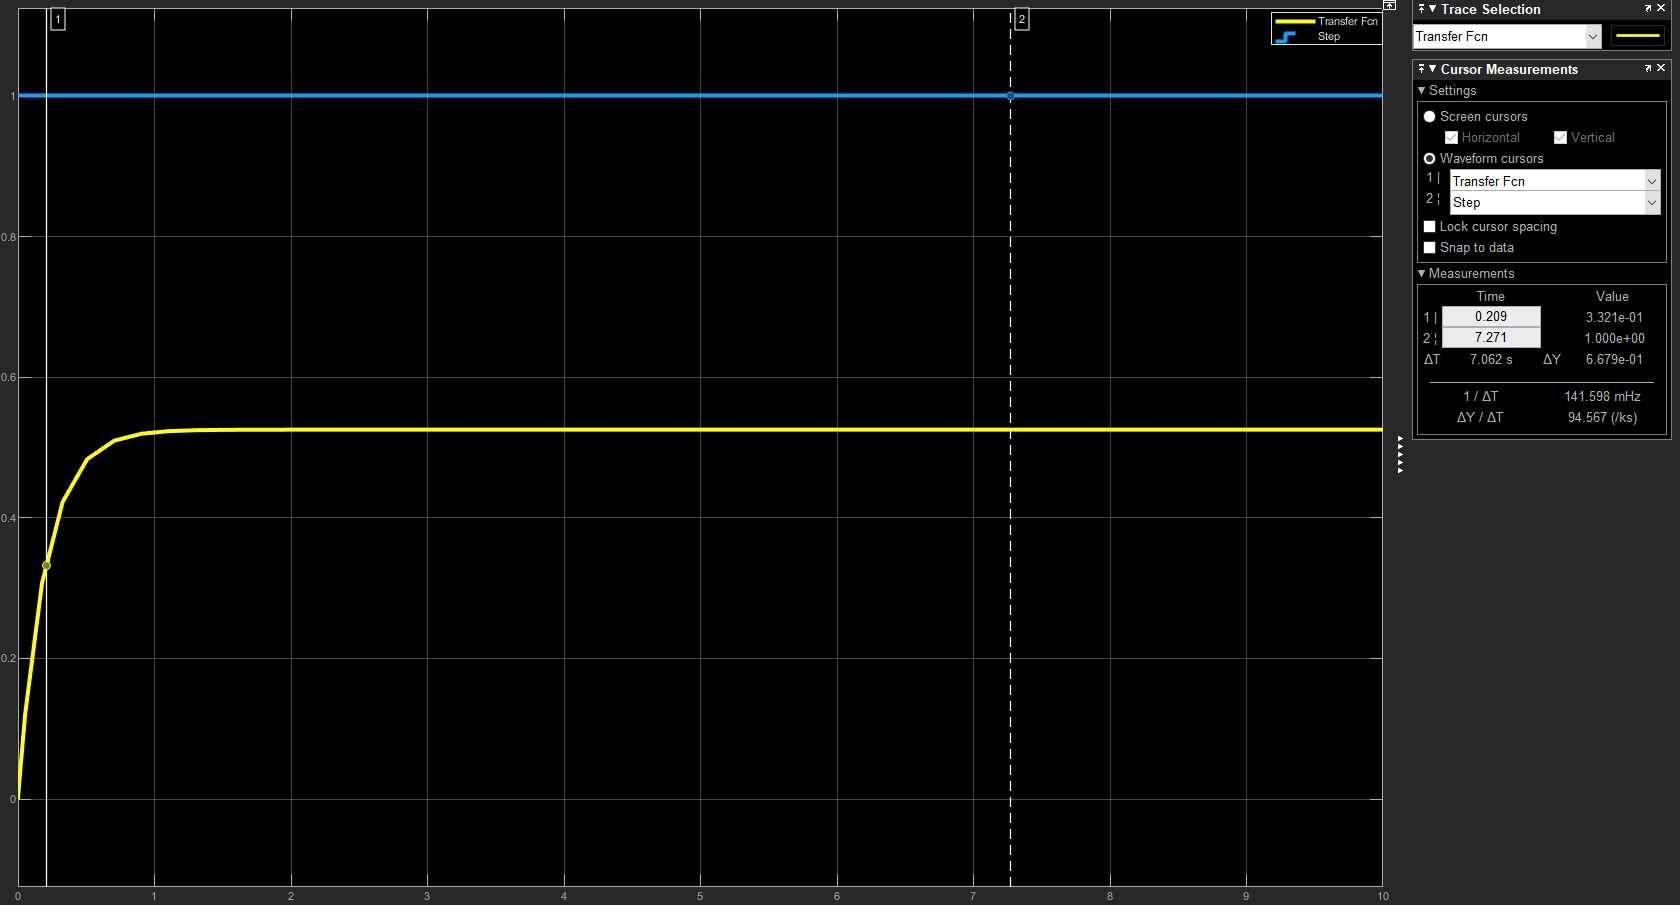
\includegraphics[width=0.7\textheight]{1_step1.1.png}
		\captionof{figure}{Step input and step response of the DC motor}
		\label{f1}
	\end{figure}

	\noindent The transfer function, $H(s)$, of the DC motor can be calculated as follows:
	\begin{align}
		\label{eq1}
		H_1(s) &= \frac{k_t}{R_a} * \frac{1}{Js + b}\nonumber\\
		&= \frac{k_t}{R_a(Js + b)} * \frac{\frac{1}{R_a J}}{\frac{1}{R_a J}}\nonumber
	\end{align}
	\begin{align}
		\therefore H_1(s) &= \frac{\frac{K_t}{R_a J}}{s + \frac{b}{J}}
	\end{align}
	\begin{align}
		H(s) &= \frac{\frac{\frac{k_t}{R_a J}}{s + \frac{b}{J}}}{1 + \frac{\frac{k_t k_m}{R_a J}}{s + \frac{b}{J}}}\nonumber\\
		&= \frac{\frac{\frac{k_t}{R_a J}}{\cancel{s + \frac{b}{J}}}}{\frac{s + \frac{b}{J} + \frac{k_t k_m}{R_a J}}{\cancel{s + \frac{b}{J}}}}\nonumber
	\end{align}
	\begin{align}
		\therefore H(s) &= \frac{\frac{k_t}{R_a J}}{s + [\frac{b}{J} + \frac{k_t k_m}{R_a J}]}
	\end{align}
	The steady state gain of the DC motor is calculated as follows:
	\begin{align}
		\lim_{s \to 0} \left[\frac{1}{s} * H(s)\right] &= \lim_{s \to 0} \left[\frac{\cancel{s} \frac{k_t}{R_a J}}{\cancel{s} \left[\cancelto{0}{s} + \left[\frac{b}{J} + \frac{k_t k_m}{R_a J}\right]\right]}\right]\nonumber\\	
		&= \lim_{s \to 0} \left[\frac{\frac{1.8350}{(3.0484)(0.2296)}}{\frac{0.0412}{0.2296} + \frac{1.8350^2}{(3.0484)(0.2296)}}\right]\nonumber
	\end{align}
	\begin{align}
		\therefore Stady\hspace{1mm} state\hspace{1mm} gain = 0.5254 \nonumber
	\end{align}
	The time constant, $\tau$, can be calculated as follows:
	\begin{align}
		\tau = \frac{1}{a}
	\end{align}
	where $a = \frac{b}{J} + \frac{k_t k_m}{R_a J}$
	\begin{align}
		\tau &= \frac{1}{\frac{b}{J} + \frac{k_t k_m}{R_a J}}\nonumber\\
		&= \frac{1}{\frac{0.0412}{0.2296} + \frac{1.8350^2}{(3.0484)(0.2296)}}\nonumber\\
		&= \frac{1}{4.99}\nonumber
	\end{align}
	\begin{align*}
		\therefore \tau = \SI{0.200}{\second}
	\end{align*}
	There is another way of finding the time constant, $\tau$.
	We know that 63.2\% of the steady state value is equal to the time constant and thus, we have the following:
	\begin{align*}
		0.632 * 0.5254 = 0.332
	\end{align*}
	Using Fig. \ref{f1}, the time constant is the x-value when the y-value = 0.332.
	Therefore, the time constant is approximately $\SI{0.200}{\second}$.\\\\
	Explicit equation for the time constant of the DC motor:
	\begin{align}
	\label{tc}
		\therefore \tau &= \frac{J}{b + \frac{k_t k_m}{R_a}}
	\end{align}
	Explicit equation for the steady state gain of the DC motor:
	\begin{align}
	\label{gain}
		\therefore k_G = \frac{R_a}{R_a b + k_t k_m}
	\end{align}
	
	\pagebreak
	\subsection{Step 2}
	Fig. \ref{f2} the Matlab Simulink simulation of the error signal of the DC motor.
	\begin{figure}[htbp]
		\centering
		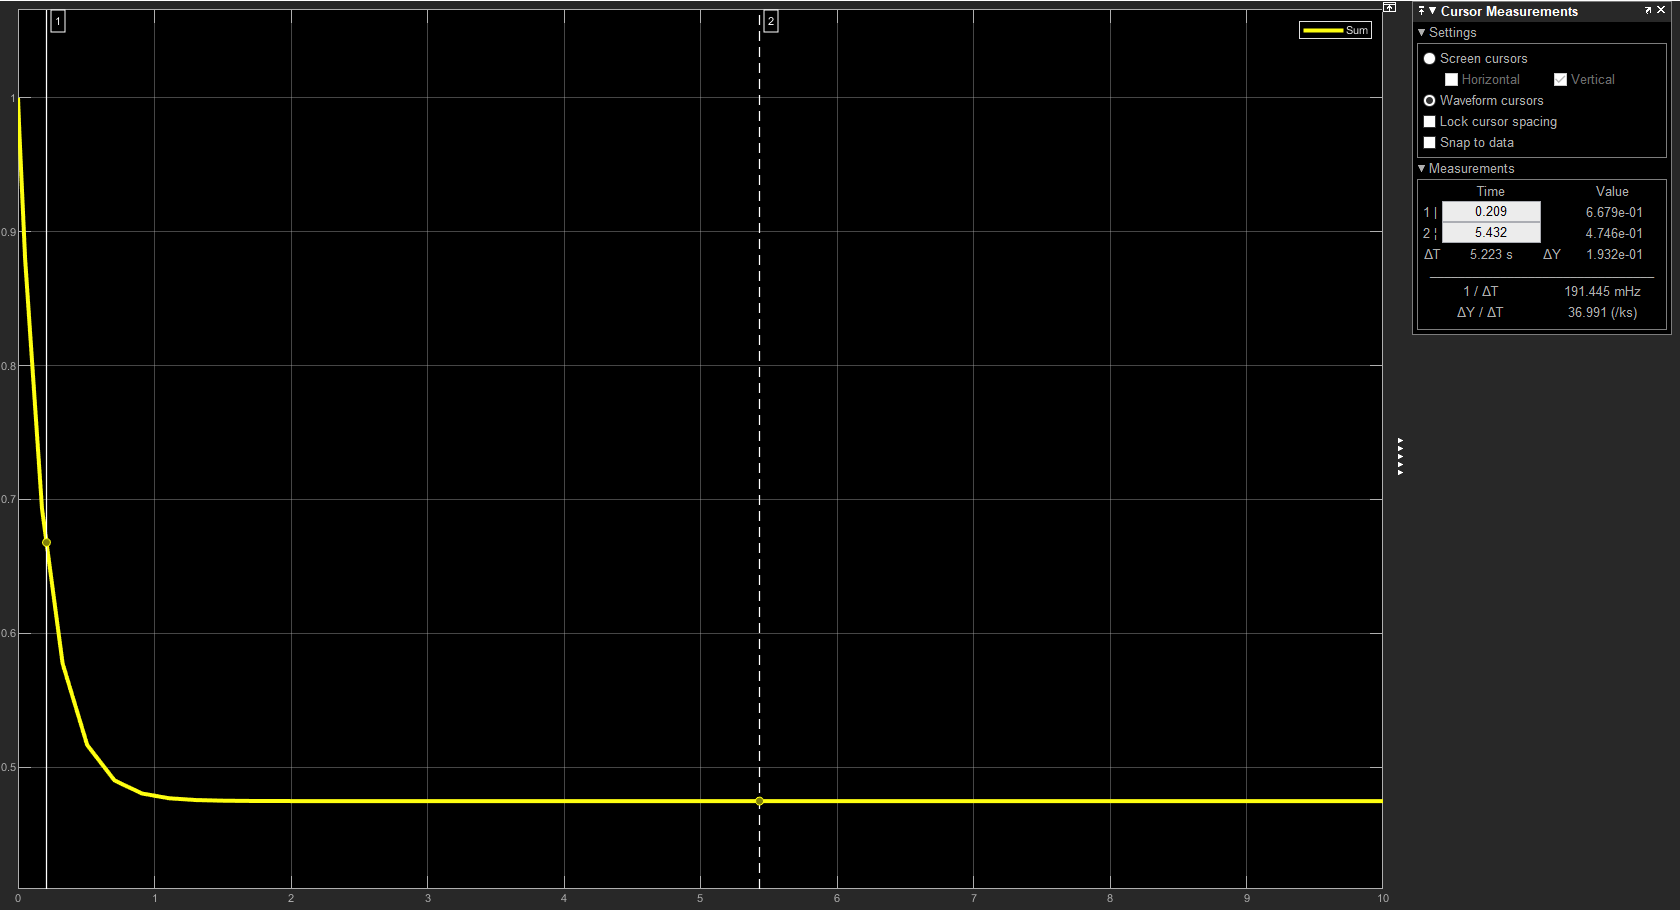
\includegraphics[width=0.7\textheight]{1_step2.1.png}
		\captionof{figure}{Time response of the error signal}
		\label{f2}
	\end{figure}

	\noindent The error signal can be calculated as follows:
	\begin{align}
		e(t) &= V_{in}(t) - \omega(t)\\
		&= 1 - 0.5254\nonumber
	\end{align}
	\begin{align*}
		\therefore e(t) = 0.4746
	\end{align*}
	\noindent It is observed that the error signal is almost half of the input signal which highlights a very important disadvantage of the open loop gain.
	Ideally, one wants the error signal to be as small as possible, if not negligible.
	
	\pagebreak
	\subsection{Step 3}
	As shown in Eq. \ref{tc}, the time constant is directly proportional to the parameter $J$ which means an increase in J would cause an increase in $\tau$, and vice verse.
	On the other hand, the gain is not affected by the changes done to parameter J as Eq. \ref{gain} does not have a parameter J in it.\\\\
	Fig. \ref{f3} and Fig. \ref{f4} show an increase and a decrease of 10\% in the time constant value respectively.
	\begin{figure}[htbp]
		\centering
		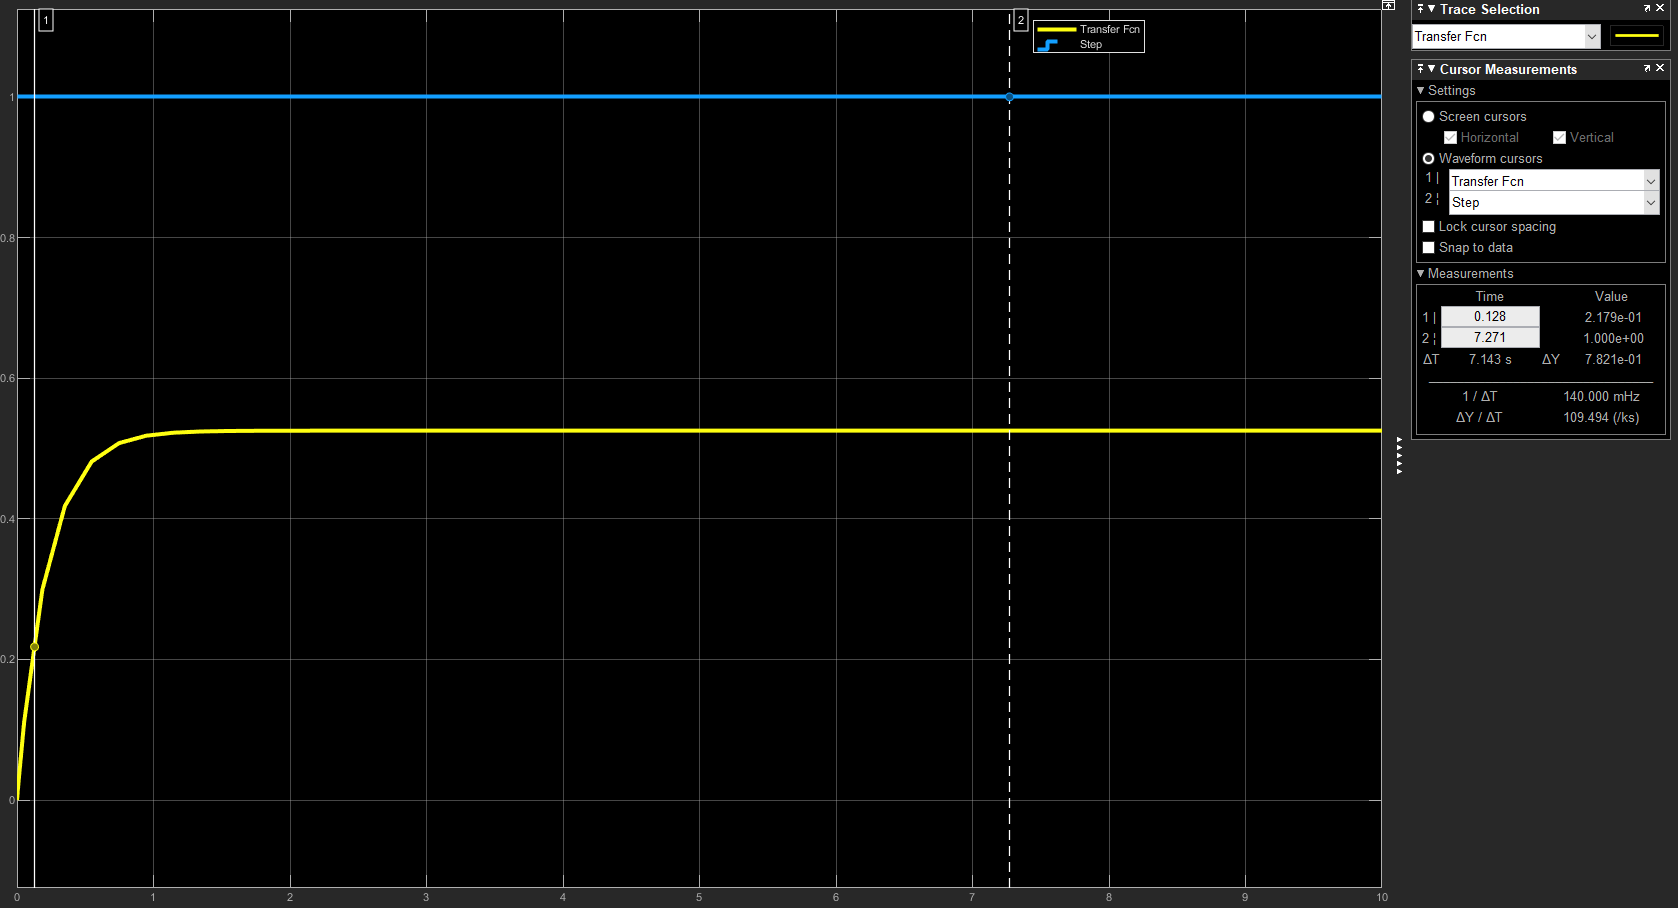
\includegraphics[width=0.6\textheight]{1_step3.1_+10.png}
		\captionof{figure}{10\% increase in time constant}
		\label{f3}
	\end{figure}	
	\begin{figure}[htbp]
		\centering
		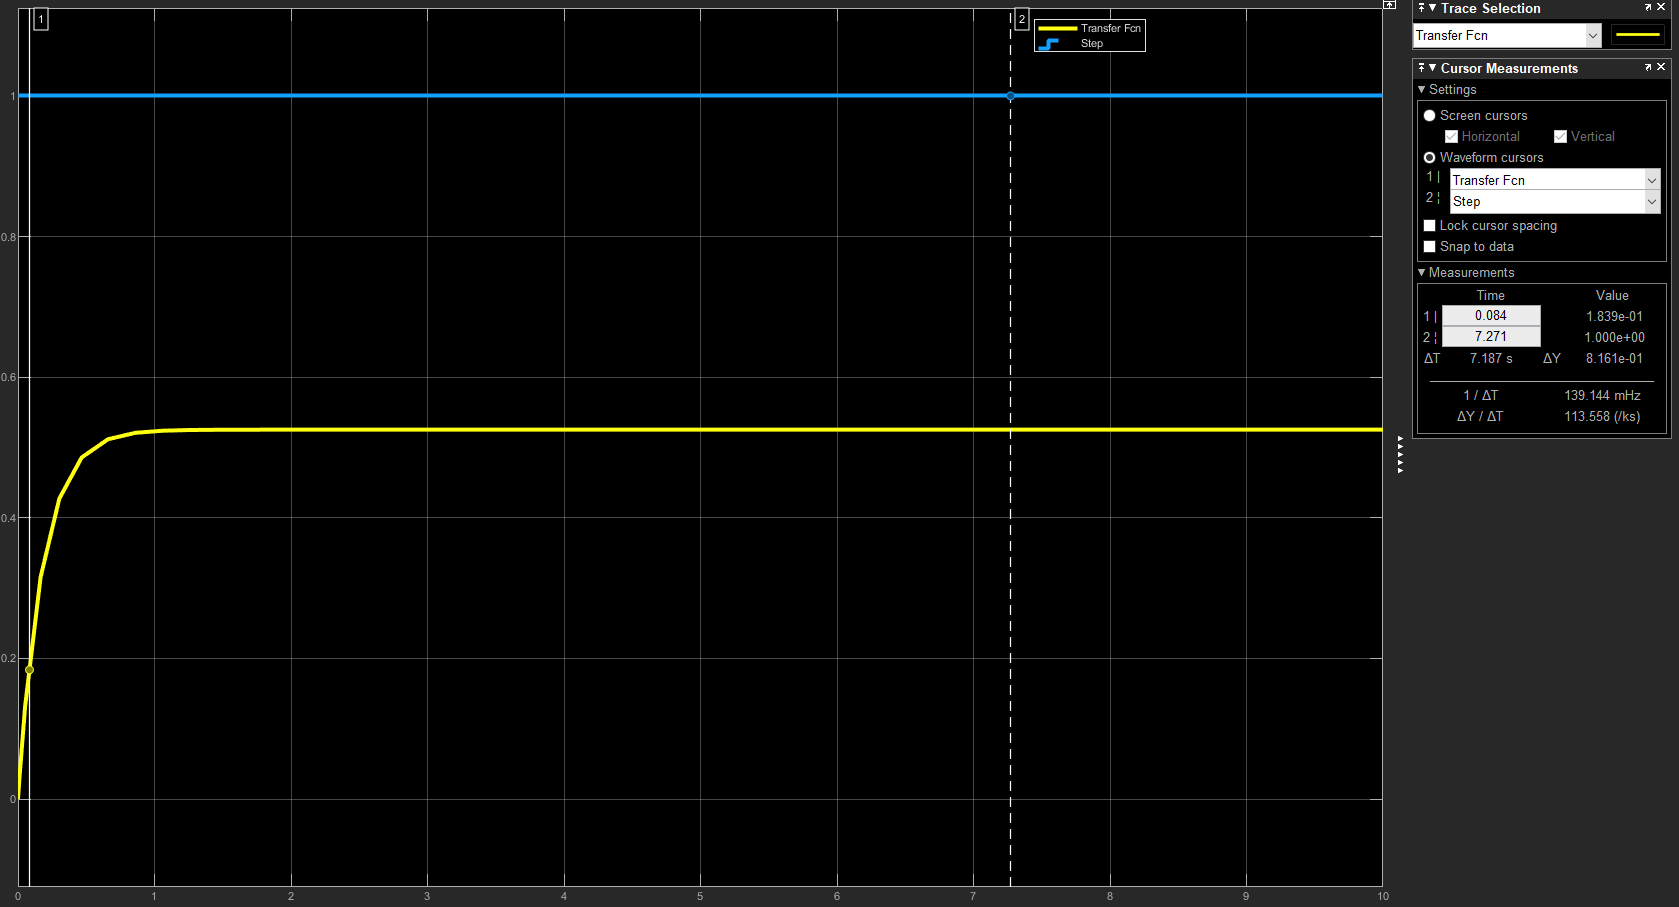
\includegraphics[width=0.6\textheight]{1_step3.1_-10.png}
		\captionof{figure}{10\% decrease in time constant}
		\label{f4}
	\end{figure}

	\pagebreak
	\subsection{Step 4}	
	The bandwidth, BW, of the transfer function can be calculated as follows:
	\begin{align}
		\label{bw}
		BW &= \frac{1}{\tau}\\
		&= \frac{1}{0.200}\nonumber
	\end{align}
	\begin{align*}
		\therefore BW = \SI{5}{\radian/\second}
	\end{align*}
	\section{The Frequency Response}
	\subsection{Step 1}
	Fig. \ref{bd} shows the bode diagram (magnitude and phase) based on the transfer function obtained using Matlab built in function.
	\begin{figure}[htbp]
		\centering
		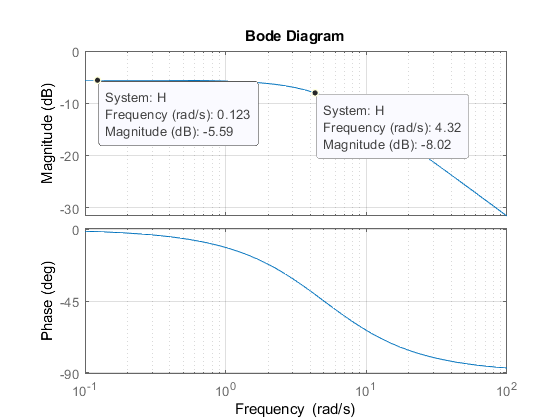
\includegraphics[width=0.7\textheight]{2_step1.png}
		\captionof{figure}{Matlab plot of the DC motor transfer function}
		\label{bd}
	\end{figure}

	\pagebreak
	\subsection{Step 2}
	Parameters shown in Table \ref{t2} are used to construct the frequency response of the system including the phase and the gain using Eq. \ref{phase} and Eq. \ref{mag}.
	\begin{align}
		\label{phase}
		\measuredangle H(j\omega) = -360 \frac{t_{\phi}}{T}
	\end{align}
	\begin{align}
		\label{mag}
		\mid H(j\omega)\mid = \frac{\Delta Y}{\Delta U}
	\end{align}
	\begin{table}[htbp]
		\centering
		\captionof{table}{Data Points}
		\begin{tabular}{|c|c|c|c|c|c|c|c|}
			\hline
			\textcolor{blue}{f (Hz)} & T (sec) & $t_\phi$ & $\Delta$Y & $\Delta$U & \textcolor{blue}{$\measuredangle$H(j$\omega$)} & $\mid$ H(j$\omega$)$\mid$ & \textcolor{blue}{20log$\mid$H(j$\omega$)$\mid$ (dB)}\\
			\hline\hline
			0.2 & 5 & 0.198 & 1.017 & 2 & -14.256 & 0.5085 & -5.8741\\
			\hline
			0.5 & 2 & 0.169 & 0.8819 & 2 & -30.42 & 0.44095 & -7.1122\\
			\hline
			1 & 1 & 0.129 & 0.6878 & 2 & -46.44 & 0.3439 & -9.2713\\ 
			\hline 
			2 & 0.5 & 0.085 & 0.4323 & 2 & -61.20 & 0.21615 & -13.3049\\
			\hline
			4 & 0.25 & 0.054 & 0.1909 & 2 & -77.76 & 0.09545 & -20.4045\\
			\hline
			6.5 & 0.153846 & 0.035 & 0.134 & 2 & -81.90 & 0.0670 & -23.4785\\
			\hline
		\end{tabular}
		\label{t2}
	\end{table}
	\subsection{Step 3}
	Fig. \ref{f44} shows the bode diagram (magnitude and phase) based on the transfer function plotted by hand using data point in Table \ref{t2}.
	\begin{figure}[htbp]
		\centering
		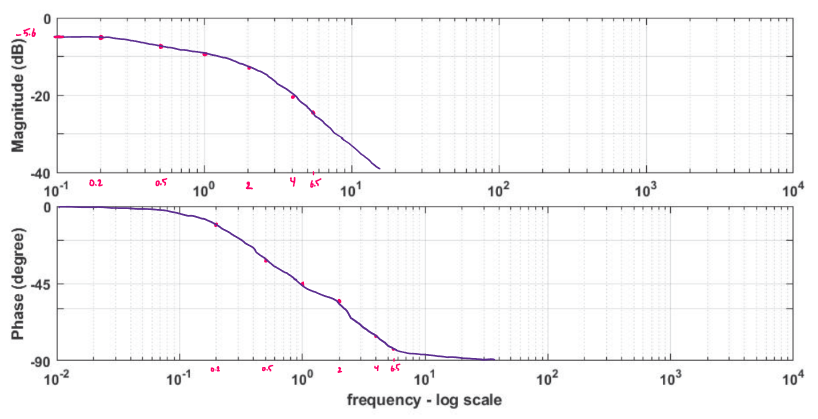
\includegraphics[width=0.7\textheight]{bodeHand.png}
		\captionof{figure}{Frequency response data points}
		\label{f44}
	\end{figure}
	
	\pagebreak
	\subsection{Step 4}
	Using Fig. \ref{f44}, the bandwidth, BW, is determined using the \SI{3}{\decibel} drop from the DC gain of the DC motor.
	\begin{align*}
		BW \approx \SI{-5.8741}{\decibel} - \SI{3}{\decibel}\nonumber
	\end{align*} 
	\begin{align*}
		BW \approx \SI{-8.8741}{\decibel}
	\end{align*}
	As shown in Eq. \ref{bw}, the general equation of the bandwidth is:
	\begin{align}
		BW &= \frac{1}{\tau}\nonumber
	\end{align}
	
	
	\subsection{Step 5}
	Based on this experiment and as shown in Fig. \ref{f2}, the open loop gain of the DC motor has a very large error signal value which is approximately 50\% of the input signal.
	This highlights a very important disadvantage of the open loop gain. The open loop gain is a type of analysis that can be used to analyze a system of dynamics. However, it should be avoided, if possible, as it has a very large error signal relative to the input signal.
	\pagebreak
	\section{References}
	[1] “Laboratory Experiment \#1: Open-Loop Analysis”, Carleton Univeristy, Ottawa, 2020.

\end{document}